\chapter{Costing}
\writer{Henri Videau}{6}
\section{Introduction}
In this chapter the current state of the ILD costing is presented. There is a strong similarity with the costing exercise for the DBD but also quite some differences. The most obvious is that the dimensions have evolved and that we try now to cost two models of ILD: the "large model" very similar to the DBD baseline and the "small model" where the outer radius of the TPC has been reduced grossly by 30cm. One important issue is to relate  the cost difference between the two models with the difference observed in their relative performances. It provides an evaluation of the impact of the size much better defined than was done with just some scaling laws. For the ECal, a version with a slightly coarser sampling is also estimated.

\section{The method}
At the time of the DBD the effort had been put on trying to have a costing coherent with the SiD estimate and the method of the accelerator had been used, i.e estimating in an "ILC currency", the ILCU. This implied making translations from different currencies using the exchange rates but mostly "Purchase Power Parities" and the difference between these two estimates may generate huge differences. At that time an ILCU was 0.97 Euros using PPP's. For todays exercise ILD decided to use Euros as counting units. When originating from Japan, like for silicon diode matrices, the prices in euros were provided by the vendors.

Except for this question the method used to establish the costing is totally similar to the DBD. It rests on the knowledge of the fabrication processes and the prices provided by the numerous prototypes built these last years.  The idea is to identify the cost drivers, often very sensitive to strong price evolution, and have a precise Work Breakdown System identifying the procurements, the tooling, the fabrication operations to estimate also the manpower, which is now most often included in the cost. The manpower may be twofold, in house manpower linked mostly to the follow-up of the operations but also to some work when the quality required requests it and the rather limited amount permits it, but we consider also industrial manpower when we do not have already industrial offers and we try to figure out a possible price by estimating the cost of a fabrication.

\section{The costing of the different sub-detectors}
The cost of each sub-detector making ILD is reviewed. This is done for both ILD models, the large and the small. As anything inside the TPC in radius is untouched, there is only one price quoted for the vertex detector, the inner tracker, the forward tracker and the forward calorimetry, this last item being composed of the Lumical, the ECal ring, the LHCal  and the BeamCal. On the contrary the costs for the TPC, the SET, the electromagnetic and hadronic calorimeters, the magnet system and the muon system are to be provided for both versions.
\subsection{The vertex detector}
This cost estimate has been provided by the note "ILD VXD and SIT Costing Estimates" by Auguste Besson and Marc Winter (January 2019) which updates the DBD. See table~\ref{vertex_cost}

\begin{table}\hspace*{-0cm}\small
\begin{tabular}[h!]{ l p{0.1\hsize}p{0.1\hsize}p{0.1\hsize} p{0.1\hsize}p{0.1\hsize}p{0.1\hsize} }
\toprule
\multicolumn{7}{ l }{{\bf Vertex detector}}\\
\midrule
Cost   & Sensors & Mechanics & Electronics & Services & Installation & Total \\
\midrule
Material    & 1152   &  452   &  486    & 770 & 100 & 2960 \\
Manpower    & 100    & 500    & 400     & 250 & 200 & 1450 \\
\midrule
Total      & 1252   &  952   &  886    & 1020 & 300 & 4410 \\
 \bottomrule
\end{tabular}
\caption{\label{vertex_cost}Elements of cost of the vertex detector in kEuros.}
\end{table}

%\begin{figure}[h!]
%\centering
%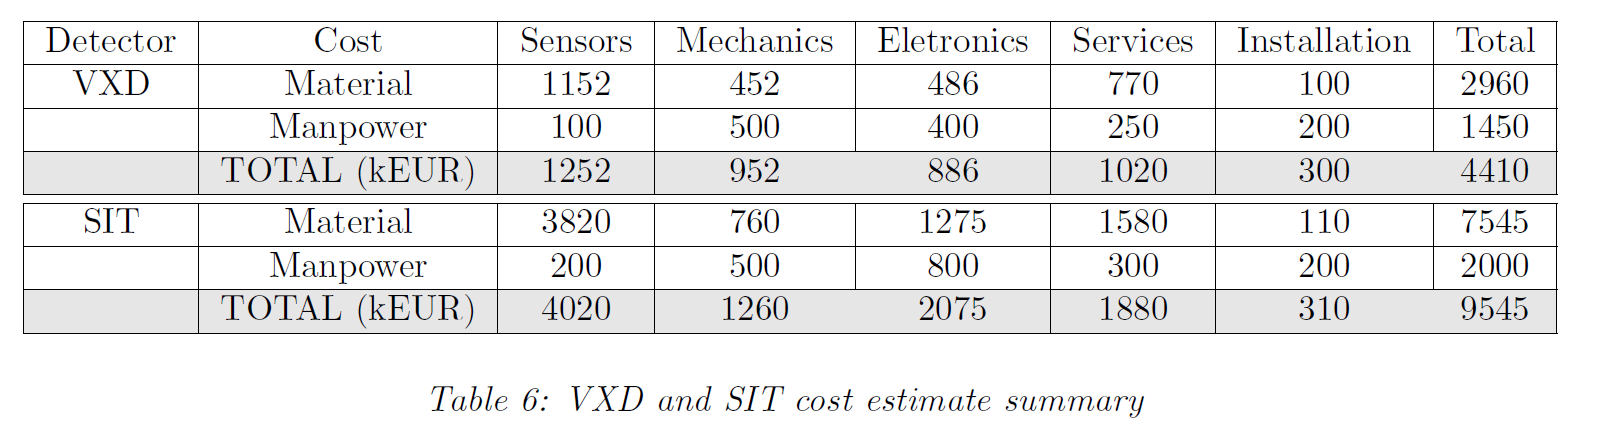
\includegraphics[width=1.0\hsize]{Costing/VXD_SIT.PNG}
%\caption{Contributions of the different items to the cost of the vertex detector.}
%\label{VXD_SIT}
%\end{figure}

\subsection{The SIT}
This is a version for a SIT using pixels in contrary to the DBD version which used strips. The costing of this version is provided by the note by A. Besson and M. Winter referenced above for the vertex. Therefore no direct comparison between the DBD cost and this one, in particular since in the DBD SIT and forward tracker were put together.
 See table~\ref{SIT_cost}. 
 \begin{table}\hspace*{-0cm}\small 
\begin{tabular}[h!]{ l p{0.1\hsize}p{0.1\hsize}p{0.1\hsize} p{0.1\hsize}p{0.1\hsize}p{0.1\hsize} }
\toprule
\multicolumn{7}{ l }{{\bf Silicon Inner Tracking}}\\
\midrule
Cost   & Sensors & Mechanics & Electronics & Services & Installation & Total \\
\midrule
Material    & 3820   &  760   & 1275    & 1580 & 110 & 7545 \\
Manpower    & 200    & 500    & 800     & 300 & 200 & 2000 \\
\midrule
Total      & 4020   &  1260   &  2075    & 1880 & 310 & 9545 \\
\bottomrule
\end{tabular}
\caption{\label{SIT_cost}Elements of cost of the SIT in kEuros.}
\end{table}

\subsection{The forward tracking}
No update since the DBD where all the elements using silicon strips (strip forward disks, SIT, SET and even ETD)  were summed together. There are 4 disks using pixel technology, the 12 other disks use strip technology. We guess a global estimate of 2MEuros expecting a  real update from Marcel Vos.

\subsection{The forward calorimeters}
In the DBD
This has been updated except for the ECal ring which remains more or less an orphan.
Since the DBD the L* has been changed and the calorimeters adjusted.
The three forward calorimeters, namely the BeamCal, the LumiCal and the LHCal have been reexamined in detail considering for each of them the mechanical elements, sensors, ASICs, front-end electronics, power supplies, data acquisition, tooling and manpower. On top of these common items LumiCal and LHCal need some specific fan-outs and the LumiCal needs a laser positioning system. This is summarised in the table~\ref{FCals_summary} for a total of 8.44 MEuros and 6 man-years equivalent to 0.48MEuros.
%\begin{figure}[h!]
%\centering
%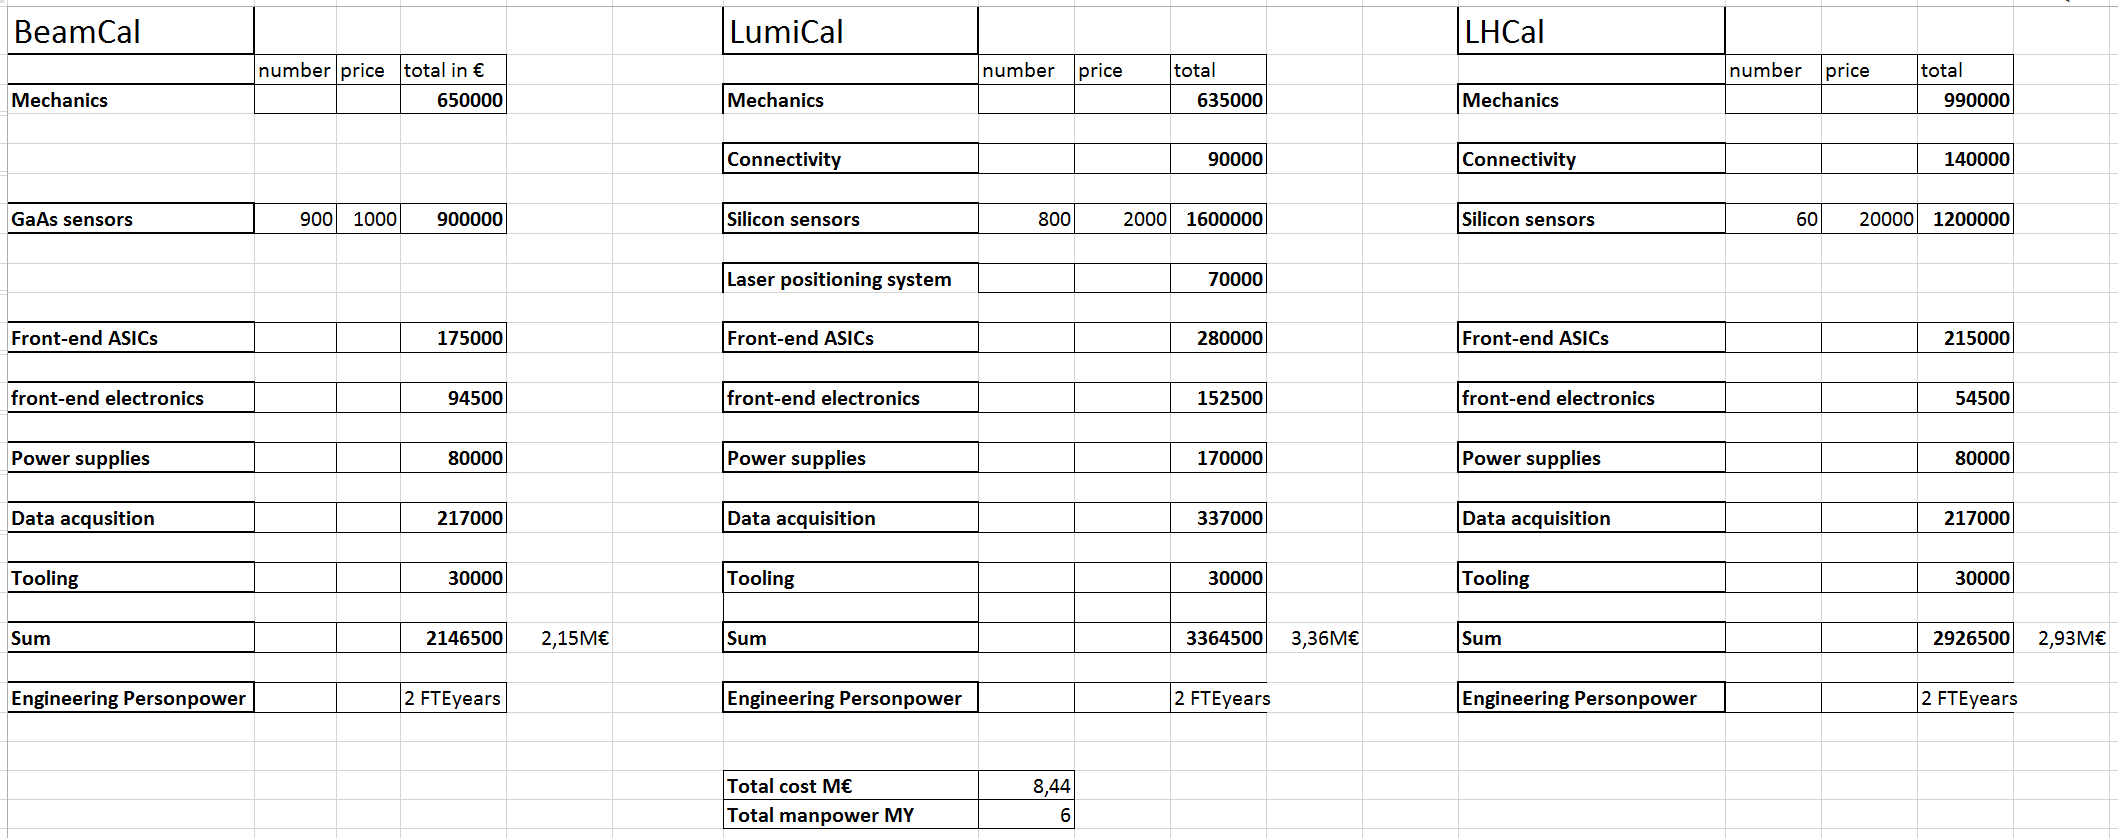
\includegraphics[width=1.\hsize]{Costing/Fcals_summary.PNG}
%\caption{Contributions of the different items to the cost of the forward calorimetry.}
%\label{Fcals_summary}
%\end{figure}

 \begin{table}\hspace*{-0cm}\small 
\begin{tabular}[h!]{ l p{0.2\hsize}p{0.2\hsize}p{0.2\hsize} }
\toprule
& BeamCal & LumiCal & LHCal \\
\midrule
Mechanics              & 650.   & 635    & 990   \\
Connectivity           &        & 90     & 140   \\
Sensors                & 900.   & 1600   & 1200  \\
Laser system           &        & 70     &       \\
Front-end ASICs        & 175.   & 280    & 215   \\
Front-end electronics  & 94.5   & 152.5  & 54.5  \\
Power supplies         & 80.    & 170    & 80    \\
Data acquisition       & 217.   & 337    & 217   \\
Tooling                & 30.    & 30     & 30    \\
\midrule
Total                  & 2150.  & 3365   & 2927  \\
\midrule
Manpower &2  &2 & 2 \\
\bottomrule
\end{tabular}
\caption{\label{FCals_summary}Elements of cost of the forward calorimeters in kEuros and manpower in MY.}
\end{table}

\subsection{The Time Projection Chamber (TPC)}
Should exist in two versions large and small. In the DBD the TPC price quoted was 35.9 MILCU which translates to 36.6 MEuros of today. This is for the large model, for the small one it may be scaled down to 27.0 MEuros. Should come sometimes dixit Paul Colas.

\subsection{The outer silicon tracker (SET)}
No real design exists. The end cap part, coined ETD, has disappeared since the DBD.The cost from the DBD is quoted 21 MILCU for both SET and ETD. A cost for the SET alone can be guessed from the areas but the number of layers is different; the SET area over the total is about 0.73 and its cost is then claimed to be 15.3 MILCU or 14.84 MEuros 2008, or about 15.5 MEuros 2018 after running the Euro. 
No cost was established for the small model. It could be scaled from the large with the ratio of the radii: 0.807, providing a cost of 12.6 MEuros.

An estimate can more accurately be derived from the cost of the CMS tracker. It is about 275kCHF per square meter of detector, silicon and mechanics. The SET area in the large model is about 52.9 square m with two layers like in the CMS tracker. That makes 14.5 MCHF to which miscellaneous things like cooling power supply and back-end electronics should be added for about 3 MCHF, say 20\%: 14.5 * 1.20 *0.89 = 15.5MEuros. 
In  the  small model the area is 42.7square m for a cost of 12.5 MEuros.

\subsection{The electromagnetic calorimeter (ECal)}
\subsubsection{The silicon version}
A costing had been done at the time of the DBD, amounting to 157 MILCU or 152MEuros, about half of it in the cost of the diode matrices. The manpower was left aside.
The new costing of the silicon electromagnetic calorimeter has been derived from a more detailed WBS in the form of about 400 lines of Excel. This WBS follows a detailed and chronological fabrication description which estimates the procurements for the different operations, the tooling needed and the operations with the amount of manpower and the duration of the operations caring about the fact that none should have a duration longer than two years. 
Almost all the difference, except for a slight tungsten price rise, between the DBD estimate and the actual large version comes from the change in the diode matrices cost estimate. For the new version we use the offer to CMS for making the HGCAL matrices. The total price, manpower excluded, reaches then 117 MEuros. In this case the manpower has also been estimated at 158 MY equivalent to 13 MEuros, bringing the total amount to 130 MEuros.

Aside the large version the small one has been also fully costed to 90MEuros + 11MEuros for the manpower making 101 MEuros. For this version a model with the small size but also with a slightly reduced number of active layers (26 instead of 30) is also costed. The impact on the resolution of the sampling is compensated by an increase of the silicon thickness to 725 micrometers. This provides a further reduction of the cost to 80 + 10 MEuros. It has to be noted that the reason for this change in sampling is more dictated by technical reasons than cost. It has also to be noted that these estimates are slightly at the advantage of the large model since most of the tooling has been estimated at the same cost for the different options.These numbers are summarised in table~\ref{ECal_summary}
\begin{table}\hspace*{-0cm}\small 
\begin{tabular}[h!]{ l p{0.2\hsize}p{0.2\hsize}p{0.2\hsize} }
\toprule
Version& Material & Manpower & Total \\
\midrule
Large model                       & 117   & 13    & 130   \\
Small model                       & 90    & 11    & 101   \\
Small model with reduced sampling & 80.   & 10    & 90  \\
\bottomrule
\end{tabular}
\caption{\label{ECal_summary}Estimates for the three versions of silicon ECal, in MEuros.}
\end{table}

As a result, the sharing between the main items is presented. If the silicon matrices cost still dominates the procurements, others are important like tungsten, printed boards, ASIcs. This sharing is presented for the small model with reduced sampling in the Figure~\ref{fig:det:ECal26_Si_cost_sharing}.
\begin{figure}[h!]
\centering
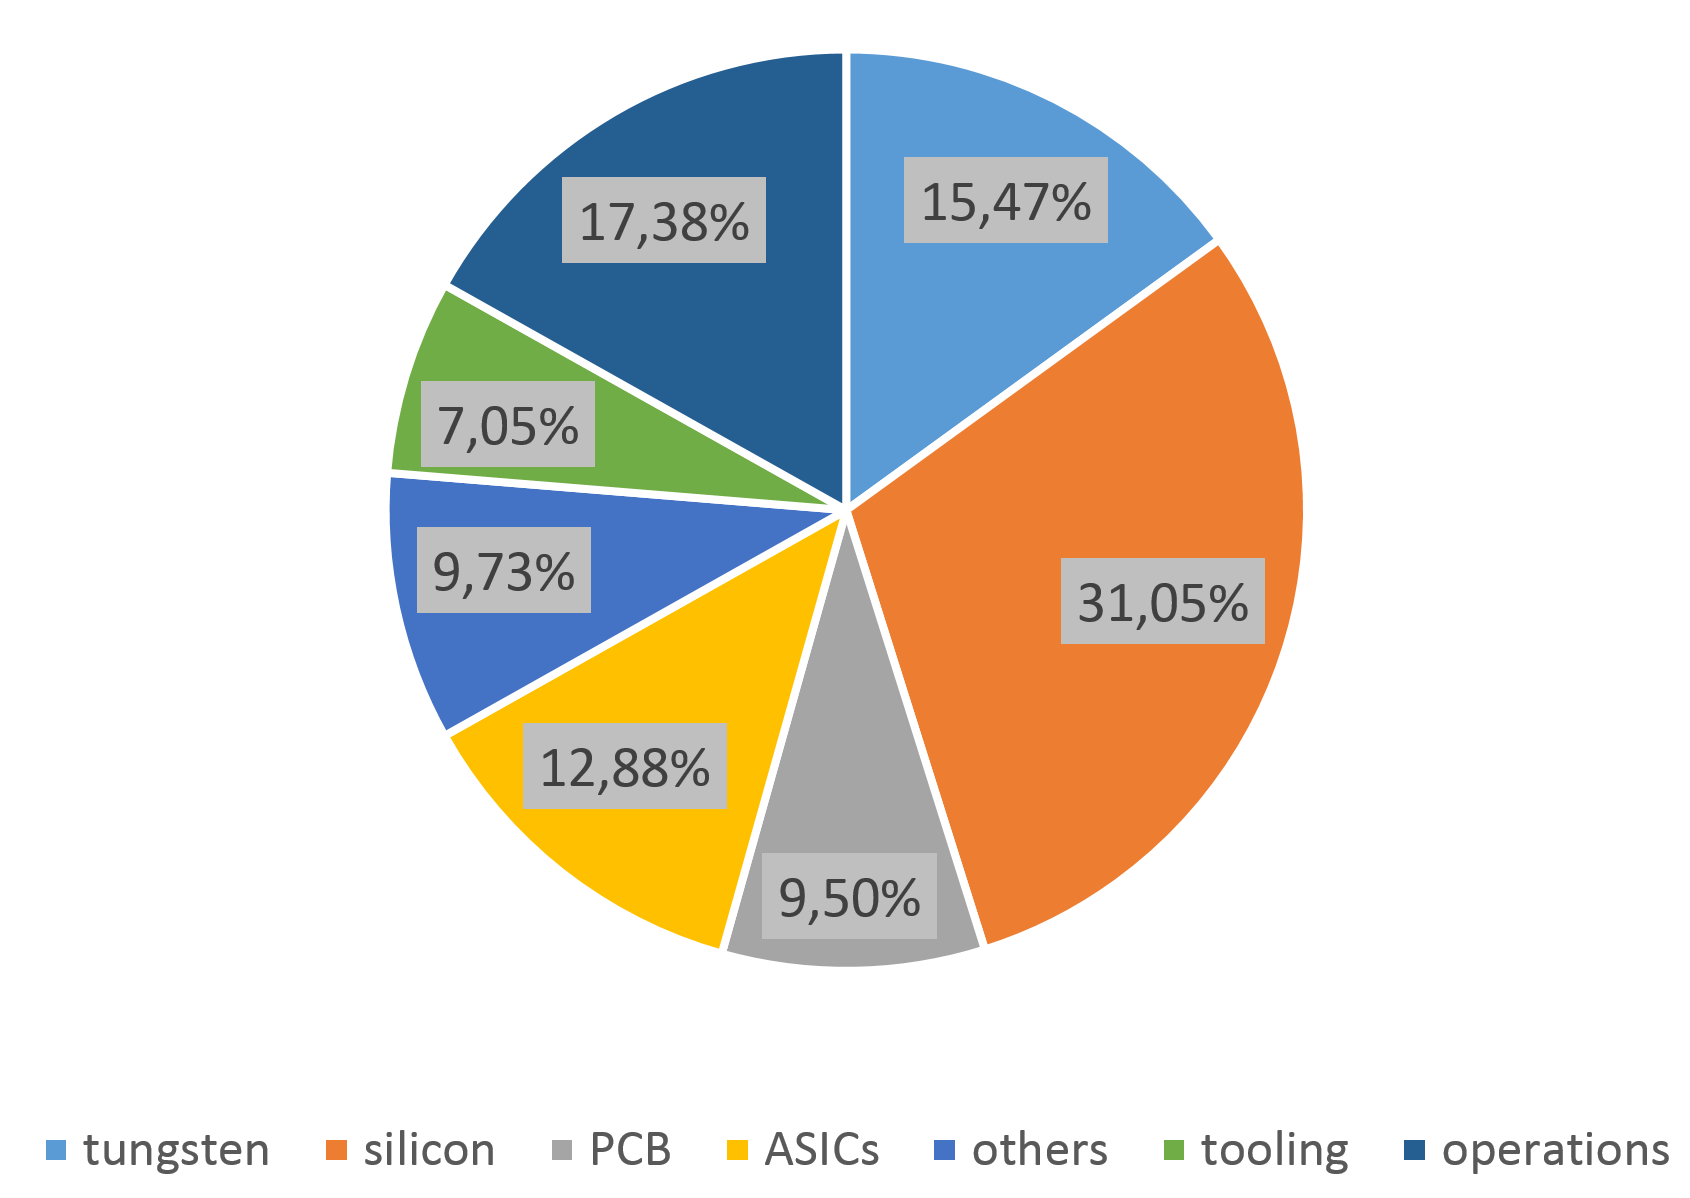
\includegraphics[width=0.8\hsize]{Costing/ECal26_Si_cost_sharing.PNG}
\caption{Contributions of the different items to the cost in the case of the "small model" with a reduced sampling.}
\label{fig:det:ECal26_Si_cost_sharing}
\end{figure}
The cost without manpower reaches 80 MEuros for 119 man-years.

\subsubsection{The scintillator version}
The cost is said to be unchanged from the DBD. It was 74 MILCU which translates to 75 MEuros after applying the price evolution. The assembly remains to be estimated as well as the manpower. No quote given for the small model but a scaling could be attempted.

\subsection{The hadron calorimeter}
\subsubsection{The analogue version}
No update for the large model, the DBD estimate appears as still valid today for essentially all the items. For the DBD the cost was 44.9 MILCU translating into 45.7 MEuros 2018 with no manpower quoted.
No detailed quote for the small model, a simple scaling corresponds to a factor 0.84 from the large to the small which cost is then 38.4, 7.3 MEuros less.

\subsubsection{The semi-digital version }
No update really available for the large model but the cost is estimated to remain similar. For the DBD the cost was 44.8 MILCU translating into 45.6 MEuros 2018 with no manpower quoted.
No real quote for the small one, a simple scaling corresponds to a factor 0.84 from the large to the small which cost is then 38.3, 7.3 MEuros less.

\subsection{The magnet}
The magnet (coil and yoke) has been revisited fully. The source for the evaluation is still the CMS documents. But the way to derive the numbers has been strongly reconsidered. The CHF costs from CMS have been converted to Euros at the exchange parity of the time, then the prices in Euros have been evolved to 2018. Therefore a comparison between the DBD and actual costs may not be totally relevant. One thing to notice though is the  strong reduction in the yoke cost. This  is due to a change in the reference cost of the iron. At the time of the DBD a price of 6ILCU/kg had been agreed upon with SiD and CLIC, in the current costing, the price payed for CMS has been used, translated in Euros and scaled today providing a price of 3.5 Euros/kg. It is not perfectly clear that this reflects fully a market price. The anti-DID is not taken here into consideration since it is not clearly defined. All this is described in detail in a note by Ch. Berriaud.

No detailed approach for costing the small version has been taken. A priori we expect the cost for the small version to be reduced but instead of 3.5T the nominal field is 4T. The impact on the coil winding and on the flux return is not trivial and it is not even clear that the cost of the magnet system does not grow.
A good approximation may be to keep the cost constant. Anyway the cost reduction linked to relaxing the stray field constraint would certainly dominate.

Some studies are going on with Japanese companies and at some point their offers shall be compared.
\begin{table}\hspace*{-0cm}\small 
\begin{tabular}[h!]{ l p{0.2\hsize}  p{0.1\hsize} }
\toprule
%\multicolumn{7}{ l }{{\bf Silicon Inner Tracking}}\\
\textbf{Magnet system} & \textbf{88}\\
\midrule
\textbf{Coil} & \textbf{29.4}\\
\midrule
Conductor and winding & 18.5\\
Internal cryogenics and suspension &  3.7\\
Suspension system & 0.3 \\
Internal instrumentation & 0.9 \\
Tooling, assembling & 5.4 \\
Qualification and partial testing & 0.6\\
\midrule
\textbf{Ancillaries for coil} & \textbf{10.6}\\
\midrule
Cryogenics and vacuum & 6.5\\
Electrical power circuits & 0.9\\
Control and safety systems& 0.6 \\
Engineering (transport to cavern) & 2.1\\
Integration in cavern& 0.3 \\
Field mapping&0,3\\
\midrule
\textbf{Yoke and vacuum tank} & \textbf{48.4}\\
\midrule
Yoke steel including works and vacuum tank& 39.6\\
Support &1.2\\
Moving system& 2.6\\
Assembly& 4.8\\
Photogrammetry and survey& 0.3 \\
\bottomrule
\end{tabular}
\caption{\label{magnet_cost}Elements of cost of the magnet system in MEuros.}
\end{table}

%\begin{figure}[h!]
%\centering
%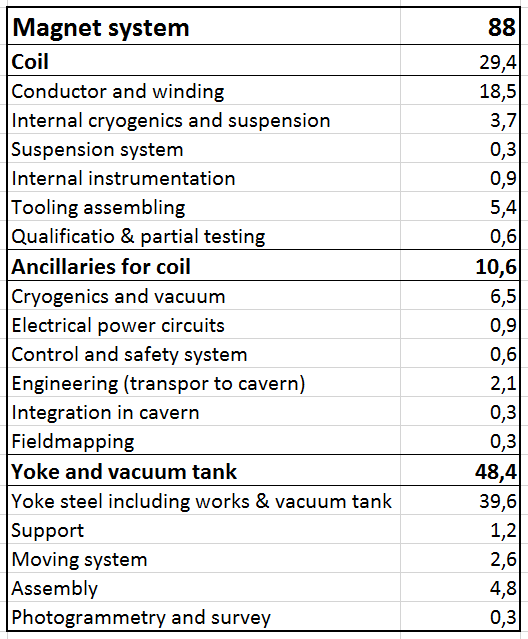
\includegraphics[width=0.5\hsize]{Detector/fig/Magnet_table.PNG}
%\caption{Magnet cost sharing. The costs are in MEuros}
%\label{fig:det:Magnet_cost_sharing}
%\end{figure}


\subsubsection{The muon system}
In the DBD it is evaluated at 6.5 MILCU equivalent to 6.6 MEuros today. But no assembly, no tooling, no manpower are evaluated. This may add 25\% to the cost growing to 8.3.

The small model can be inferred by a simple scaling where the end cap chambers are scaled by the square of the radii and the barrel ones by the radius. This provides an estimate of 6 + 1.55 Meuros for the small  model.

\section{The global cost of each of the models.}
The information developed in the preceding subsections can be summed up in a table presenting the two models side by side.
\begin{table}[h!]\hspace*{-0cm}\small
\begin{tabular}{ l p{0.2\hsize}p{0.1\hsize}p{0.2\hsize} p{0.2\hsize}p{0.1\hsize}}
\toprule
\bf {Item}& \bf {Large model} & \bf manpower&  \bf {Small model}&\bf manpower \\
\midrule
Vertex detector    & 2.96 &1.45  &  idem &idem \\
Silicon Internal Tracker & 7.55&2.0 & idem&idem\\
Forward tracker    & 1.5  &0.5  & idem &idem  \\
LumiCal & 3.37 & 0.16& idem&idem\\
ECal ring & 0&0 & idem&idem\\
LHCal & 2.93 &0.16&idem& idem\\
BeamCal & 2.15 &0.16& idem&idem\\
\midrule
Time Projection Chamber & 36.6 & 0&27.0&0\\
Silicon External Tracker & \it12.6& 1.9&10.8&1.7\\
Si Electromagnetic Calorimeter & 117 & 13.0 & 90. & 11.\\
Sc Electromagnetic Calorimeter & 75 & ? & ? & ?\\
A. Hadron Calorimeter & \it45.7 & ? & \it38.4 & ?\\
sD. Hadron Calorimeter & \it45.6 & ? & \it38.3 & ?\\
Coil and ancillaries &  40 & 0& idem & 0\\
Yoke and vacuum tank &  48.4 & 0& idem & 0 \\
Muon system  &  \it6.6 & 1.7 & 6 & 1.55\\
\midrule
Total      & 327   &  21  & 281 & 18.7  \\
\midrule
Total with MP     & 348   &    & 299.7 & 0  \\
 \bottomrule
\end{tabular}
\caption{\label{cost_summary}Elements of cost of ILD in MEuros. The numbers in italic are from the DBD. The manpower has been translated from man-years to euros.}
\end{table}

\section{Comparison with the DBD cost estimate.}
 When comparing the prices above to the DBD's 392MILCU it should be recalled that the new prices are in Euros, that for the DBD ECal it was a mix between the scintillator and the silicon versions  and that globally the manpower cost was left out. The sharing between the sub-detectors is shown for the different versions in the figures~\ref{fig:det:DBD_cost_sharing}, ~\ref{Costing:Large_cost_sharing}, ~\ref{Costing:Small_cost_sharing}. Using a reduced sampling in the ECal reduces the cost by 10MEuros, last figure. The increase in the fraction of the ECal comes from the fact that purely the silicon version is quoted here and with manpower. 
\begin{figure}[h!]
\centering
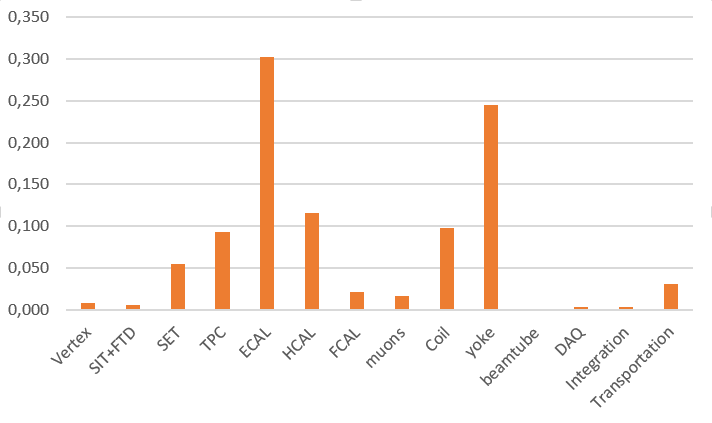
\includegraphics[width=0.8\hsize]{Detector/fig/DBD_cost_sharing.PNG}
\caption{ILD cost sharing as it is in the DBD}
\label{fig:det:DBD_cost_sharing}
\end{figure}

\begin{figure}[h!]
\centering
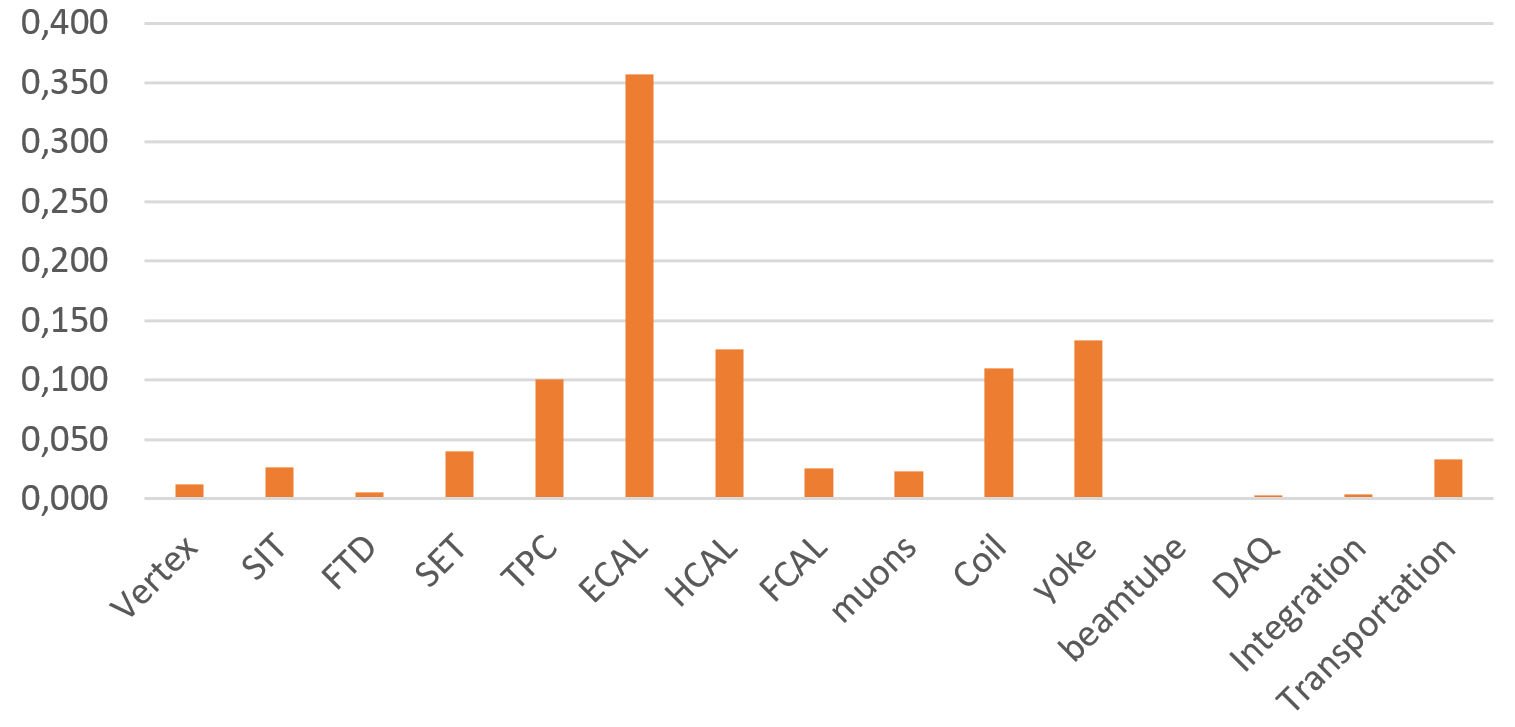
\includegraphics[width=0.8\hsize]{Costing/Large_cost_sharing.PNG}
\caption{ILD cost sharing in the large model}
\label{Costing:Large_cost_sharing}
\end{figure}

\begin{figure}[h!]
\centering
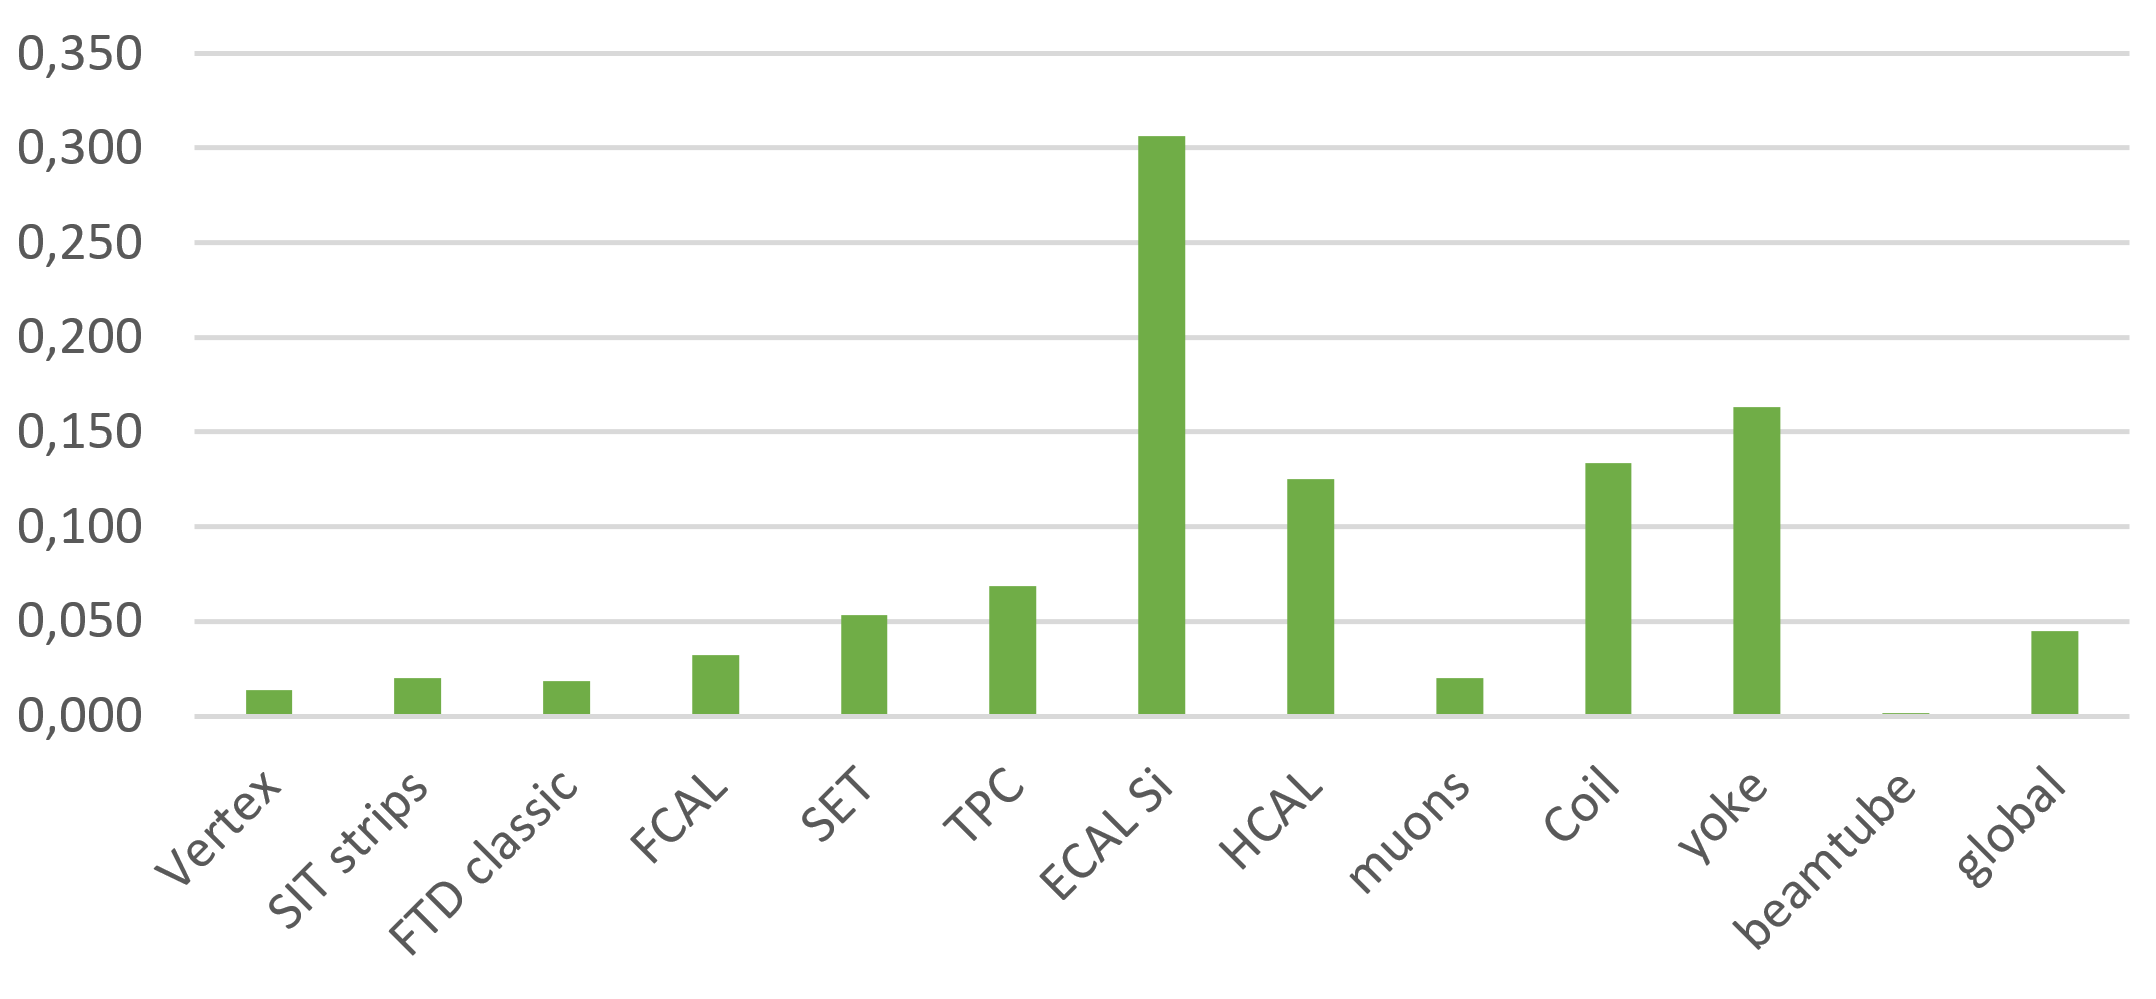
\includegraphics[width=0.8\hsize]{Costing/Small_cost_sharing.PNG}
\caption{ILD cost sharing in the small (26) model}
\label{Costing:Small_cost_sharing}
\end{figure}
